\begin{titlepage}
\begin{center}

% Upper part of the page. The '~' is needed because \\
% only works if a paragraph has started.
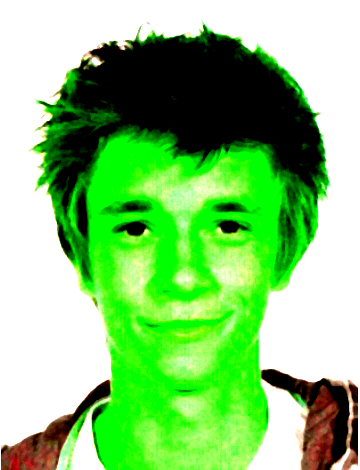
\includegraphics[width=0.2\textwidth]{img/max_vert}~\\[1cm]

\textsc{\LARGE École Polytechnique de Louvain}\\[1.5cm]

\textsc{\Large Rapport de projet}\\[0.5cm]

% Title
\HRule \\[0.4cm]
{ \huge \bfseries Modélisation et réalisation \\ d’un haut-parleur \\[0.4cm] }

\HRule \\[1.5cm]

% Authors, tutor and coordinator
\begin{minipage}{0.45\textwidth}
\begin{flushleft} \large
\emph{Auteurs:}\\
\quad Noëlla \textsc{Bola Malanda}\\
\quad Giulia \textsc{de Dorlodot}\\
\quad Maxime \textsc{Hanot}\\
\quad Victor \textsc{Lecomte}\\
\quad Timothée \textsc{Malengreau}\\
\quad Bastien \textsc{Tagnon}
\end{flushleft}
\end{minipage}
\qquad \qquad
\begin{minipage}{0.3\textwidth}
\begin{flushleft} \large
\emph{Tuteur:} \\
\quad Britney \textsc{Spears}\\
\emph{Coordonnateur:}\\
\quad Piotr \textsc{Sobieski}\\
\vspace{3\baselineskip}
\end{flushleft}
\end{minipage}

\vfill

% Bottom of the page
{\large \today}

\end{center}
\end{titlepage}
